\documentclass{article}\usepackage[]{graphicx}\usepackage[]{color}
%% maxwidth is the original width if it is less than linewidth
%% otherwise use linewidth (to make sure the graphics do not exceed the margin)
\makeatletter
\def\maxwidth{ %
  \ifdim\Gin@nat@width>\linewidth
    \linewidth
  \else
    \Gin@nat@width
  \fi
}
\makeatother

\definecolor{fgcolor}{rgb}{0.345, 0.345, 0.345}
\newcommand{\hlnum}[1]{\textcolor[rgb]{0.686,0.059,0.569}{#1}}%
\newcommand{\hlstr}[1]{\textcolor[rgb]{0.192,0.494,0.8}{#1}}%
\newcommand{\hlcom}[1]{\textcolor[rgb]{0.678,0.584,0.686}{\textit{#1}}}%
\newcommand{\hlopt}[1]{\textcolor[rgb]{0,0,0}{#1}}%
\newcommand{\hlstd}[1]{\textcolor[rgb]{0.345,0.345,0.345}{#1}}%
\newcommand{\hlkwa}[1]{\textcolor[rgb]{0.161,0.373,0.58}{\textbf{#1}}}%
\newcommand{\hlkwb}[1]{\textcolor[rgb]{0.69,0.353,0.396}{#1}}%
\newcommand{\hlkwc}[1]{\textcolor[rgb]{0.333,0.667,0.333}{#1}}%
\newcommand{\hlkwd}[1]{\textcolor[rgb]{0.737,0.353,0.396}{\textbf{#1}}}%
\let\hlipl\hlkwb

\usepackage{framed}
\makeatletter
\newenvironment{kframe}{%
 \def\at@end@of@kframe{}%
 \ifinner\ifhmode%
  \def\at@end@of@kframe{\end{minipage}}%
  \begin{minipage}{\columnwidth}%
 \fi\fi%
 \def\FrameCommand##1{\hskip\@totalleftmargin \hskip-\fboxsep
 \colorbox{shadecolor}{##1}\hskip-\fboxsep
     % There is no \\@totalrightmargin, so:
     \hskip-\linewidth \hskip-\@totalleftmargin \hskip\columnwidth}%
 \MakeFramed {\advance\hsize-\width
   \@totalleftmargin\z@ \linewidth\hsize
   \@setminipage}}%
 {\par\unskip\endMakeFramed%
 \at@end@of@kframe}
\makeatother

\definecolor{shadecolor}{rgb}{.97, .97, .97}
\definecolor{messagecolor}{rgb}{0, 0, 0}
\definecolor{warningcolor}{rgb}{1, 0, 1}
\definecolor{errorcolor}{rgb}{1, 0, 0}
\newenvironment{knitrout}{}{} % an empty environment to be redefined in TeX

\usepackage{alltt}[11pt]
\usepackage{amsmath}
\usepackage{amssymb}
\usepackage{geometry}
\usepackage{graphicx}
\usepackage{bm}
\usepackage{url}
\usepackage{hyperref}
\usepackage{enumerate}
\usepackage{fullpage}
\IfFileExists{upquote.sty}{\usepackage{upquote}}{}
\begin{document}

\setlength\parindent{0pt}

\textbf{SLR Practice Problem}\\

Many people believe that gender, weight, drinking habits, and many other factors are much more important in predicting blood alcohol content (BAC) than simply considering the number of drinks a person consumed. Here we examine data from sixteen student volunteers at Ohio State University who each drank a randomly assigned number of cans of beer. These students were evenly divided between men and women, and they differed in weight and drinking habits. Thirty minutes later, a police officer measured their blood alcohol content (BAC) in grams of alcohol per deciliter of blood.  Below is the R output from fitting a simple linear regression model to this data.  A scatter plot with the least squares line is also shown below. 

\begin{knitrout}\scriptsize
\definecolor{shadecolor}{rgb}{0.969, 0.969, 0.969}\color{fgcolor}\begin{kframe}
\begin{alltt}
\hlkwd{library}\hlstd{(openintro)}
\hlkwd{data}\hlstd{(}\hlstr{"bac"}\hlstd{)}
\hlstd{lm1} \hlkwb{<-} \hlkwd{lm}\hlstd{(BAC} \hlopt{~} \hlstd{Beers,} \hlkwc{data} \hlstd{= bac)}
\hlkwd{summary}\hlstd{(lm1)}
\end{alltt}
\begin{verbatim}
## 
## Call:
## lm(formula = BAC ~ Beers, data = bac)
## 
## Residuals:
##       Min        1Q    Median        3Q       Max 
## -0.027118 -0.017350  0.001773  0.008623  0.041027 
## 
## Coefficients:
##              Estimate Std. Error t value Pr(>|t|)    
## (Intercept) -0.012701   0.012638  -1.005    0.332    
## Beers        0.017964   0.002402   7.480 2.97e-06 ***
## ---
## Signif. codes:  0 '***' 0.001 '**' 0.01 '*' 0.05 '.' 0.1 ' ' 1
## 
## Residual standard error: 0.02044 on 14 degrees of freedom
## Multiple R-squared:  0.7998,	Adjusted R-squared:  0.7855 
## F-statistic: 55.94 on 1 and 14 DF,  p-value: 2.969e-06
\end{verbatim}
\begin{alltt}
\hlkwd{par}\hlstd{(}\hlkwc{mar}\hlstd{=}\hlkwd{c}\hlstd{(}\hlnum{4}\hlstd{,}\hlnum{4}\hlstd{,}\hlnum{1}\hlstd{,}\hlnum{1}\hlstd{),} \hlkwc{cex}\hlstd{=}\hlnum{0.8}\hlstd{)} \hlcom{# adjust margins and font size}
\hlkwd{plot}\hlstd{(bac}\hlopt{$}\hlstd{Beers, bac}\hlopt{$}\hlstd{BAC,} \hlkwc{xlab}\hlstd{=}\hlstr{"Cans of beer"}\hlstd{,} \hlkwc{ylab}\hlstd{=}\hlstr{"BAC (grams /  deciliter)"}\hlstd{)}
\hlkwd{abline}\hlstd{(lm1)}
\end{alltt}
\end{kframe}
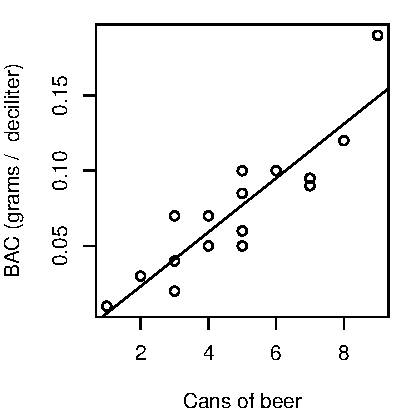
\includegraphics[width=\maxwidth]{figure/unnamed-chunk-1-1} 

\end{knitrout}

\clearpage
\begin{enumerate}[(a)]
\item Describe the association between number of cans of beer and BAC.
\item What are the explanatory and response variables for the linear regression model?
\item Write the equation for the least squares line.
\item Interpret the slope and the intercept in context.
\item What is the predicted BAC for a person that drank 5 cans of beer?
\item A student in this data set drank 9 beers and had a measured BAC of 0.19. Calculate the residual for this student. %student 3
\item Interpret the coefficient of determination ($R^2$).
\item Do the data provide strong evidence that drinking more cans of beer is associated with an increase in blood alcohol content?  State the null and alternative hypotheses, report the test statistic and $p$-value (from the \texttt{summary()} command), and state your conclusion.
\item Calculate a 95\% confidence interval for $\beta_1$.
\item Do the data provide evidence that the intercept is significantly different than 0?  State the null and alternative hypotheses, report the test statistic and $p$-value (from the \texttt{summary()} command), and state your conclusion.
\item Calculate a 95\% confidence interval for $\beta_0$.
\item Are the conditions for linear regression reasonably satisfied?  In your assessment, comment on the plot of the residuals versus number of cans of beer ($x$), and the QQ plot of the residuals shown below.
\end{enumerate}

\begin{knitrout}\scriptsize
\definecolor{shadecolor}{rgb}{0.969, 0.969, 0.969}\color{fgcolor}\begin{kframe}
\begin{alltt}
\hlkwd{par}\hlstd{(}\hlkwc{mfrow}\hlstd{=}\hlkwd{c}\hlstd{(}\hlnum{1}\hlstd{,}\hlnum{2}\hlstd{),} \hlkwc{cex}\hlstd{=}\hlnum{0.7}\hlstd{)}
\hlkwd{plot}\hlstd{(bac}\hlopt{$}\hlstd{Beers,} \hlkwd{resid}\hlstd{(lm1),} \hlkwc{xlab}\hlstd{=}\hlstr{"Number of beers"}\hlstd{,} \hlkwc{ylab}\hlstd{=}\hlstr{"Residuals"}\hlstd{)}
\hlkwd{abline}\hlstd{(}\hlkwc{h}\hlstd{=}\hlnum{0}\hlstd{)}
\hlkwd{qqnorm}\hlstd{(}\hlkwd{resid}\hlstd{(lm1))}
\hlkwd{qqline}\hlstd{(}\hlkwd{resid}\hlstd{(lm1))}
\end{alltt}
\end{kframe}
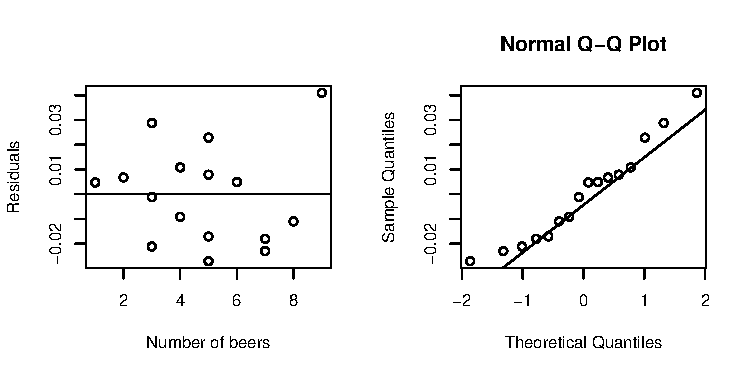
\includegraphics[width=\maxwidth]{figure/unnamed-chunk-2-1} 

\end{knitrout}






\end{document}
